% ==============================================================================
% 第 8 章：列表 (Chapter 8: Lists)
% ==============================================================================

\chapter{列表}
\label{sec:ch08_lists}

你在此前很可能从未接触过\term{自引用定义}（self-referential definition）。你的语文老师肯定会对这类定义敬而远之，而许多数学课程在涉及这类定义时往往语焉不详。然而，程序员绝不能含糊其辞，他们的工作要求绝对的精确性。虽然一般而言一个定义可能包含多处对自身的引用，但本章将从最有用的例子——列表（list）开始，展示仅需一次自引用的优雅范例。

引入列表还极大地丰富了我们所能研究的应用类型。本章将通过丰富的实例精心建立你的直觉，同时为下一章修订程序设计配方提供充足的动机——下一章将系统阐述如何针对自引用数据定义编写函数。

\section{创建列表}
\label{sec:ch08_creating_lists}

我们每个人在日常生活中都在不停地列清单。在去超市购物前，我们会写下一张采购清单；有些人每天早晨都会列一份待办事项（to-do list）；在十二月，许多孩子会准备一份圣诞愿望清单；为了筹办聚会，我们会整理一份邀请宾客的名单。将信息组织成列表形式，早已融入我们生活的方方面面。

既然信息天然呈现为列表的形式，我们就必须学会如何在 BSL 中将此类列表表示为数据。事实上，正因为列表至关重要，BSL 像支持笛卡尔坐标点（\code{posn}）一样，内置了对创建和操作列表的原生支持。但与坐标点不同的是，列表的数据定义永远由你自己来决定。不过我们先从最基础的开始：创建列表。

当构建一个列表时，我们总是从\term{空列表}（empty list）开始。在 BSL 中，空列表表示为：
\begin{lstlisting}[language=BSL]
'()
\end{lstlisting}
读作“empty”，即“空列表”的简写。与 \code{\#true} 或 \code{5} 一样，\code{'()} 也是一个常量。当我们向列表中添加元素时，就会构造出一个新的列表；在 BSL 中，\code{cons} 操作正是用于此目的。例如：
\begin{lstlisting}[language=BSL]
(cons "Mercury" '())
\end{lstlisting}
它由空列表 \code{'()} 和字符串 \code{"Mercury"} 构造出一个包含一个元素的列表。图~\ref{fig:building_a_list} 以我们之前展示结构体相同的图示方法展示了这个列表。\code{cons} 方框有两个字段：\code{first}（首元素）和 \code{rest}（其余部分）。在此例中，\code{first} 字段存放 \code{"Mercury"}，而 \code{rest} 字段存放 \code{'()}。

\begin{figure}[htbp]
  \centering
  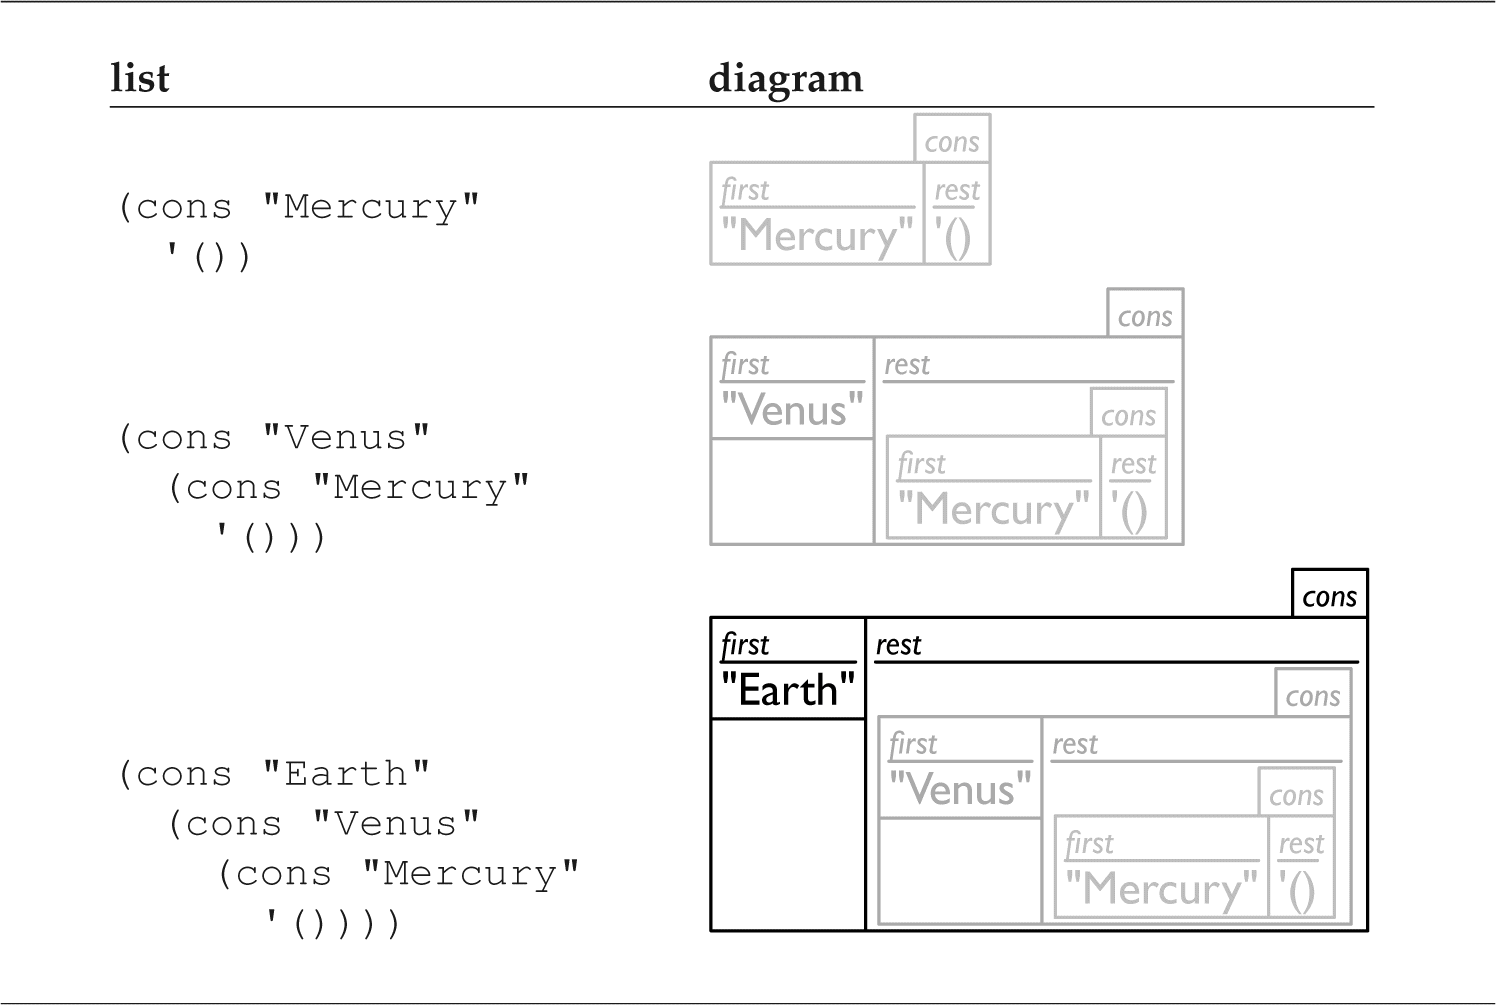
\includegraphics[width=0.75\textwidth]{images/00164.png}
  \caption{构建列表}
  \label{fig:building_a_list}
\end{figure}

一旦有了一个包含单个元素的列表，我们就可以再次使用 \code{cons} 来构造包含两个元素的列表。例如：
\begin{lstlisting}[language=BSL]
(cons "Venus" (cons "Mercury" '()))
\end{lstlisting}
再如：
\begin{lstlisting}[language=BSL]
(cons "Earth" (cons "Mercury" '()))
\end{lstlisting}

图~\ref{fig:building_a_list} 的中间一行展示了如何想象包含两个元素的列表。它同样是一个具有两个字段的方框，但此时其 \code{rest} 字段中包含着另一个方框。实际上，它所包含的正是在同一张图中上一行所示的方框。

最后，我们构造一个包含三个元素的列表：
\begin{lstlisting}[language=BSL]
(cons "Earth" (cons "Venus" (cons "Mercury" '())))
\end{lstlisting}

图~\ref{fig:building_a_list} 的最后一行展示了这个三元素列表。其 \code{rest} 字段包含一个方框，而该方框中又嵌套着另一个方框。因此，随着我们创建列表，我们实际上是在“大盒套中盒，中盒套小盒”。初看之下这或许有些奇特，但它就像俄罗斯套娃或我们生日时收到的层层嵌套的礼物盒。唯一的区别在于，BSL 程序中列表嵌套的深度，远胜于任何工匠能制造的物理套盒。

由于即便是高超的画师也很难手绘极深嵌套的结构，计算机科学家改用\term{盒与箭头图}（box-and-arrow diagrams）。图~\ref{fig:drawing_a_list} 展示了如何重排图~\ref{fig:building_a_list} 的最后一行。每个 \code{cons} 结构变成一个独立的方框。如果 \code{rest} 字段过于复杂无法直接在方框内画出，我们就画一个圆点，并引出一条带箭头的线指向它所包含的方框。根据方框的排布方式，可以得到两类图示：图~\ref{fig:drawing_a_list} 顶行展示的是按照方框\textbf{创建的先后顺序}排列的；底行展示的则是按照它们被 \code{cons} \textbf{组合的逻辑顺序}排列的。因此，第二种图示能让你一目了然地看出对该列表调用 \code{first} 会得到什么，无论列表有多长。出于这个原因，程序员更青睐第二种排布方式。

\begin{figure}[htbp]
  \centering
  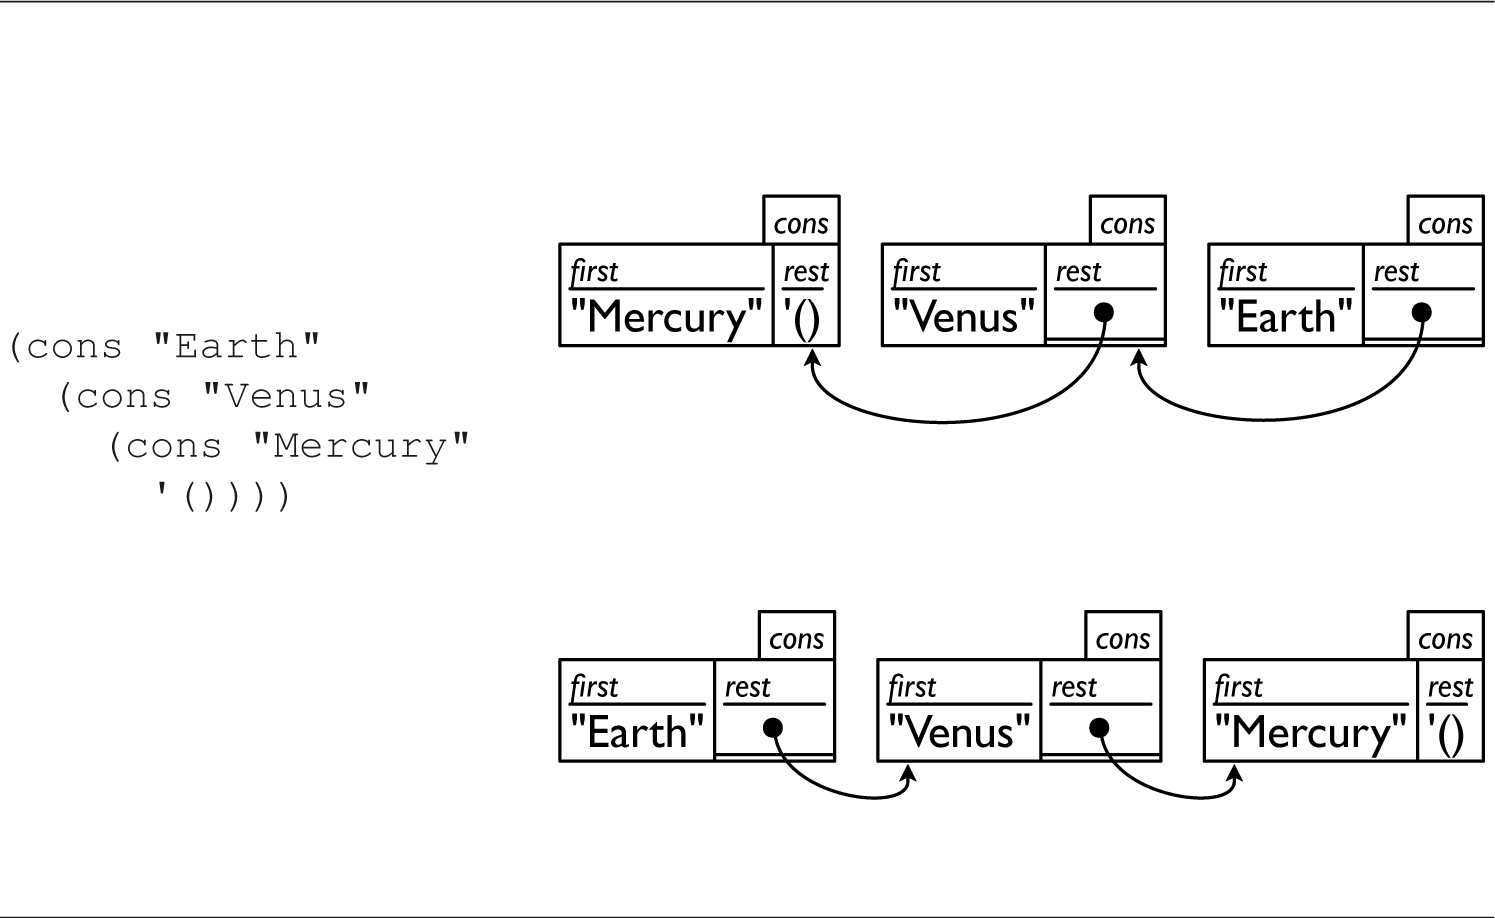
\includegraphics[width=0.75\textwidth]{images/00165.png}
  \caption{绘制列表}
  \label{fig:drawing_a_list}
\end{figure}

\begin{exercise}{创建基础列表}{129}
创建表示下列内容的 BSL 列表：
\begin{enumerate}
  \item 天体列表，至少包含太阳系中的所有行星；
  \item 一餐的食物清单，例如：牛排（steak）、薯条（french fries）、豆子（beans）、面包（bread）、水（water）、布里奶酪（Brie cheese）以及冰淇淋（ice cream）；
  \item 颜色列表。
\end{enumerate}
参考图~\ref{fig:building_a_list} 和图~\ref{fig:drawing_a_list}，绘制这些列表的方框图表示。你更喜欢哪种绘制方式？
\end{exercise}

你也可以创建数字列表。下面是一个包含 10 个一位数字（0 到 9）的列表：
\begin{lstlisting}[language=BSL]
(cons 0
  (cons 1
    (cons 2
      (cons 3
        (cons 4
          (cons 5
            (cons 6
              (cons 7
                (cons 8
                  (cons 9 '()))))))))))
\end{lstlisting}

构建这个列表需要 10 次 \code{cons} 构造以及一个 \code{'()}。对于一个包含三个任意数字的列表，例如：
\begin{lstlisting}[language=BSL]
(cons 1 (cons 2 (cons 3 '())))
\end{lstlisting}
我们需要三次 \code{cons}。

一般而言，列表并不要求所包含的值都是同一种类型，它可以包含任意类型的值：
\begin{lstlisting}[language=BSL]
(cons "Robin" (cons 12 (cons #true '())))
\end{lstlisting}

这个列表的第一个元素是字符串，第二个是数字，最后一个是布尔值。你可以将此列表视作一条包含三项数据的人事记录：雇员姓名、在公司的工龄、以及雇员是否通过公司加入了医疗保险。或者，你也可以将其视为游戏中虚拟玩家的某种状态。如果没有数据定义，你根本无从得知这些数据究竟代表什么。

\begin{notebox}[结构体 vs 列表]
如果某个数据用于表示包含\textbf{固定数量}组件的信息记录，应该优先使用结构体（structure type）；如果数据包含的项数是\textbf{任意大小}的，才应该使用列表。
\end{notebox}

下面是一个涉及 \code{cons} 的最初步的数据定义：
\begin{lstlisting}[language=BSL]
; 3LON 是包含三个数字的列表：
;   (cons Number (cons Number (cons Number '())))
; 解释：三维空间中的一个点
\end{lstlisting}

当然，这个数据定义使用 \code{cons} 的方式与使用结构体构造器并无二致，在某种意义上，\code{cons} 就是一个特殊的构造器。但该定义未能展示的是：如何形成\textbf{任意长度}的列表——包含 0 个项、1 个项、2 个项、10 个项，抑或 1,438,901 个项的列表。

让我们再做一次尝试：
\begin{lstlisting}[language=BSL]
; List-of-names 是以下之一：
; -- '()
; -- (cons String List-of-names)
; 解释：按姓氏排列的受邀宾客名单
\end{lstlisting}

深吸一口气，再仔细读一遍。这是你遇到过的最不同寻常的定义之一——在此之前，你从未见过一个\textbf{引用自身}的定义。它甚至看起来令人怀疑是否讲得通。毕竟，如果你对语文老师说“桌子就是桌子”来定义“桌子”，最可能得到的回答是“荒谬！”，因为自引用定义并没有阐明一个词汇的含义。

然而，在计算机科学和程序设计中，自引用定义扮演着核心角色；只要稍加严谨规范，此类定义是完全合情合理的。在这里，“合情合理”意味着我们可以将此数据定义用于其既定目的：生成属于该定义类别的\textbf{数据示例}，或者检查给定的某块数据是否属于所定义的类别。从这个角度来看，\code{List-of-names} 的定义完全经得起检验：
\begin{itemize}
  \item 首先，根据分项分类中的第一条分支，我们可以生成 \code{'()} 作为第一个例子。
  \item 有了 \code{'()} 作为 \code{List-of-names} 的一个已知元素，利用第二条分支很容易构造出第二个例子：
\begin{lstlisting}[language=BSL]
(cons "Findler" '())
\end{lstlisting}
  这里我们使用了字符串 \code{"Findler"} 和已确认为 \code{List-of-names} 的 \code{'()}，根据第二条规则生成了一个新的数据。
  \item 依此类推，我们可以生成更多此类单元素列表：
\begin{lstlisting}[language=BSL]
(cons "Flatt" '())
(cons "Felleisen" '())
(cons "Krishnamurthi" '())
\end{lstlisting}
  \item 虽然上述列表都只包含一个名字，但根据第二条规则，我们完全可以使用已有的单元素列表来生成包含更多名字的列表：
\begin{lstlisting}[language=BSL]
(cons "Felleisen" (cons "Findler" '()))
\end{lstlisting}
  这段数据属于 \code{List-of-names}，因为 \code{"Felleisen"} 是一个字符串，而 \code{(cons "Findler" '())} 已被证实属于 \code{List-of-names}。
\end{itemize}

\begin{exercise}{宾客名单验证}{130}
创建一个属于 \code{List-of-names} 且包含 5 个字符串的元素。参考图~\ref{fig:building_a_list} 绘制该列表的方框图表示。

请解释为什么：
\begin{lstlisting}[language=BSL]
(cons "1" (cons "2" '()))
\end{lstlisting}
是 \code{List-of-names} 的一个元素，而 \code{(cons 2 '())} 则不是。
\end{exercise}

\begin{exercise}{布尔值列表的数据定义}{131}
为表示布尔值列表给出数据定义。该类别包含任意长度的布尔值列表。
\end{exercise}

\section{什么是 '()，什么是 cons}
\label{sec:ch08_what_is_empty_and_cons}

让我们稍作停顿，仔细审视 \code{'()} 和 \code{cons}。正如前面提到的，\code{'()} 只是一个常量。与 \code{5} 或 \code{"this is a string"} 等常量相比，它看起来更像是一个函数名或变量；但若与 \code{\#true} 和 \code{\#false} 相比，就不难看出它确实只是 BSL 中用于表示空列表的符号常量。

在我们之前的求值规则中，\code{'()} 是一种全新的\textbf{原子值}（atomic value），与数字、布尔值、字符串等任何其他类型截然不同。它也不是复合值（如 \code{posn}）。事实上，\code{'()} 是如此独特，以至于它自身构成了一个独立的数值类别。因此，该类别配备了一个专用的谓词，仅识别 \code{'()} 而不识别任何其他值：
\begin{lstlisting}[language=BSL]
; Any -> Boolean
; 判断给定值是否为 '()
(define (empty? x) ...)
\end{lstlisting}

如同所有谓词一样，\code{empty?} 可以应用于 BSL 值世界中的任何值。当且仅当应用于 \code{'()} 时，它产生 \code{\#true}：
\begin{replbox}
> (empty? '())
#true
> (empty? 5)
#false
> (empty? "hello world")
#false
> (empty? (cons 1 '()))
#false
> (empty? (make-posn 0 0))
#false
\end{replbox}

接下来我们转向 \code{cons}。目前所见的一切都在提示：\code{cons} 是一个构造器，就像结构体类型定义所引入的构造器一样。更准确地说，\code{cons} 似乎是一个具有两个字段的结构体的构造器：第一个字段存放任意类型的值，第二个字段存放类似列表的值。以下定义将这一思想转换为 BSL 代码：
\begin{lstlisting}[language=BSL]
(define-struct pair [left right])

; ConsPair 是一个结构体：
;   (make-pair Any Any)

; Any Any -> ConsPair
(define (our-cons a-value a-list)
  (make-pair a-value a-list))
\end{lstlisting}

唯一的区别在于，\code{our-cons} 的第二个参数接受所有可能的 BSL 值，而真正的 \code{cons} 则不然，如下面的交互实验所示：
\begin{replbox}
> (cons 1 2)
cons: second argument must be a list, but received 1 and 2
\end{replbox}

换言之，\code{cons} 实际上是一个\term{带类型检查的函数}（checked function，如第 6 章所述）。这促使我们对定义进行细化：
\begin{lstlisting}[language=BSL]
; ConsOrEmpty 是以下之一：
; -- '()
; -- (make-pair Any ConsOrEmpty)
; 解释：ConsOrEmpty 是所有列表构成的类别

; Any Any -> ConsOrEmpty
(define (our-cons a-value a-list)
  (cond
    [(empty? a-list) (make-pair a-value a-list)]
    [(pair? a-list) (make-pair a-value a-list)]
    [else (error "cons: second argument must be a list")]))
\end{lstlisting}

既然 \code{cons} 是一个带类型检查的构造函数，你可能会好奇该如何从生成的结构体中提取各个部分。毕竟第 5 章曾说明，针对结构体编程必须借助选择器（selector）。由于 \code{cons} 结构有两个字段，因此存在两个选择器：\code{first} 和 \code{rest}。它们同样很容易基于我们的 \code{pair} 结构体来定义：
\begin{lstlisting}[language=BSL]
; ConsOrEmpty -> Any
; 提取列表的首元素
(define (our-first a-list)
  (if (empty? a-list)
      (error "first: expects a non-empty list")
      (pair-left a-list)))

; ConsOrEmpty -> ConsOrEmpty
; 提取列表除首元素外的其余部分
(define (our-rest a-list)
  (if (empty? a-list)
      (error "rest: expects a non-empty list")
      (pair-right a-list)))
\end{lstlisting}

请停下来思考片刻，自行定义 \code{our-rest}！

如果你的程序能够直接访问 \code{pair} 结构体的定义，就很容易构造出在 \code{right} 字段中既不包含 \code{'()} 也不包含另一个 \code{pair} 的非法实例。无论这种不良实例是故意还是无意创建的，它们往往会以怪异的方式破坏函数和程序。因此，BSL 特意隐藏了 \code{cons} 底层的结构体类型定义以避免这些问题。

图~\ref{fig:list_primitives} 总结了本节的核心内容。关键洞见在于：\code{'()} 是一个独一无二的原子值，而 \code{cons} 是一个产生列表值的带类型校验构造器。此外，\code{first}、\code{rest} 和 \code{cons?} 不过是常规谓词和选择器的特殊命名。因此，本章所讲授的并非一种创造数据的新方式，而是一种\textbf{阐明数据定义的新方式}。

\begin{figure}[htbp]
  \centering
  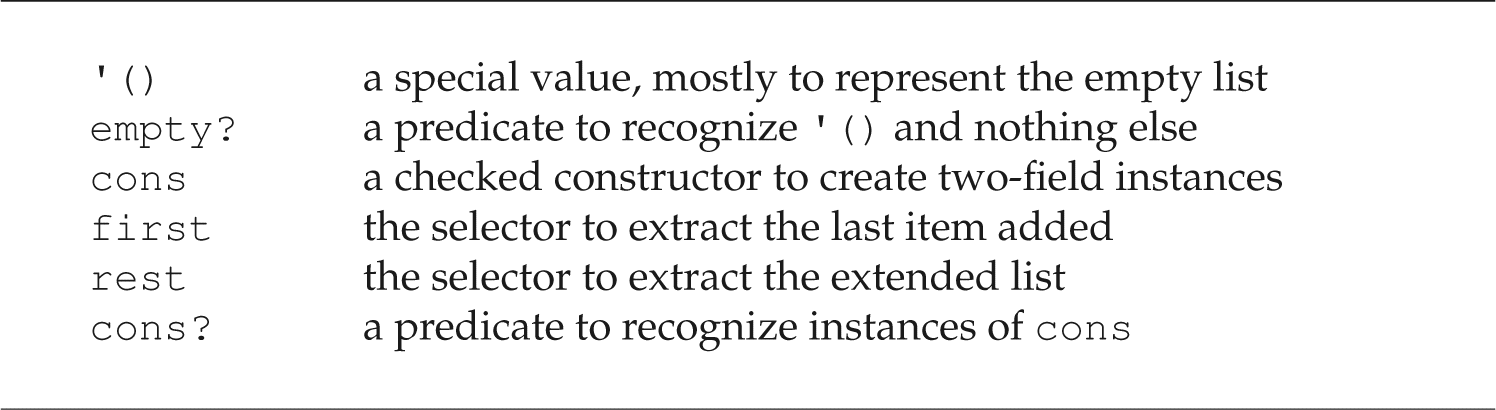
\includegraphics[width=0.8\textwidth]{images/00170.png}
  \caption{列表基本原语}
  \label{fig:list_primitives}
\end{figure}

\section{针对列表编程}
\label{sec:ch08_programming_with_lists}

假设你正在用一个列表记录你的朋友名单，并且这个列表已经变得非常庞大，以至于你需要一个程序来判断某个名字是否在名单中。为了让这一想法具象化，我们将其表述为一个例题：

\begin{notebox}[应用场景例题]
你正在为一款新手机开发通讯录功能。手机用户会在各种场合更新和查阅该通讯录。当前你的任务是：设计一个函数，接受该联系人列表，并判断其中是否包含名字 \code{"Flatt"}。
\end{notebox}

一旦解决了这个例题，我们便可将其推广为一个能在列表中查找\textbf{任意}名字的通用函数。

上一节中的 \code{List-of-names} 数据定义恰好适合用来表示待搜索的名字列表。接下来完成函数的前期材料（签名、目的说明和桩函数）：
\begin{lstlisting}[language=BSL]
; List-of-names -> Boolean
; 判断 "Flatt" 是否出现在 a-list-of-names 中
(define (contains-flatt? a-list-of-names)
  #false)
\end{lstlisting}

虽然 \code{a-list-of-names} 能准确表达输入参数的含义，但略显冗长，因此我们通常将其简写为 \code{alon}。

按照设计配方的常规步骤，接下来构造能够体现函数目的的示例。首先考虑最简单的输入：空列表 \code{'()}。既然该列表不包含任何字符串，它显然不包含 \code{"Flatt"}：
\begin{lstlisting}[language=BSL]
(check-expect (contains-flatt? '()) #false)
\end{lstlisting}

然后考虑只包含单个元素的列表：
\begin{lstlisting}[language=BSL]
(check-expect (contains-flatt? (cons "Findler" '())) #false)
(check-expect (contains-flatt? (cons "Flatt" '())) #true)
\end{lstlisting}
在第一种情况下，结果为 \code{\#false}，因为列表中的唯一元素并非 \code{"Flatt"}；在第二种情况下结果为 \code{\#true}。

最后，给出一个更通用的多元素列表示例：
\begin{lstlisting}[language=BSL]
(check-expect (contains-flatt? (cons "A" (cons "Flatt" (cons "C" '())))) #true)
\end{lstlisting}
停下来思考一下：请构造一个包含多个名字但返回值为 \code{\#false} 的示例！

停下来深吸一口气，运行一下测试。函数头是一个“桩”（dummy）定义；你构造了示例并转成了测试；更棒的是，其中某些测试居然通过了！虽然它们通过的原因纯属巧合，但确实通过了。如果一切清晰，请继续往下读。

第四步是根据数据定义设计\term{函数模板}（template）。因为字符串列表的数据定义包含\textbf{两个分支}，所以函数体必须是一个包含\textbf{两个分支}的 \code{cond} 表达式。这两个条件用于确定函数接收到的是哪一类列表：
\begin{lstlisting}[language=BSL]
(define (contains-flatt? alon)
  (cond
    [(empty? alon) ...]
    [(cons? alon) ...]))
\end{lstlisting}
在第二个分支中，我们也可以使用 \code{else} 代替 \code{(cons? alon)}。

我们可以通过依次考察每个 \code{cond} 分支为模板增加更多提示信息。具体而言，设计配方建议：如果对应的输入类别由复合数据构成，则在该分支中列出所有的选择器表达式。在我们的例子中，\code{'()} 不包含组件；而非空列表由一个字符串和另一个字符串列表构成。因此，我们在模板中加入 \code{(first alon)} 和 \code{(rest alon)}：
\begin{lstlisting}[language=BSL]
(define (contains-flatt? alon)
  (cond
    [(empty? alon) ...]
    [(cons? alon)
     (... (first alon) ... (rest alon) ...)]))
\end{lstlisting}

现在进入第五步：编写函数体。我们从模板出发，逐个处理每个 \code{cond} 分支：
\begin{itemize}
  \item 如果 \code{(empty? alon)} 为真，输入为空列表，函数必须产生 \code{\#false}。
  \item 第二个分支中 \code{(cons? alon)} 为真。模板提醒我们存在第一个字符串 \code{(first alon)} 以及列表的其余部分 \code{(rest alon)}。考察形如下式的例子：
\begin{lstlisting}[language=BSL]
(cons "A" (cons ... '()))
\end{lstlisting}
  函数就像人类一样，必须将第一个元素与 \code{"Flatt"} 进行比较。在此例中第一个是 \code{"A"} 而非 \code{"Flatt"}，因此比较结果为 \code{\#false}。如果第一个元素是 \code{"Flatt"}，则比较结果为 \code{\#true}。这意味着 \code{cond} 的第二行应该包含比较首元素是否等于 \code{"Flatt"} 的表达式：
\begin{lstlisting}[language=BSL]
(string=? (first alon) "Flatt")
\end{lstlisting}
\end{itemize}

此外，如果该比较得到 \code{\#true}，函数可以直接返回 \code{\#true}；如果比较结果为 \code{\#false}，我们还剩下列表的其余部分：\code{(rest alon)}。显然，此时函数还无法得出最终结论，因为答案取决于后续元素是什么。换言之，如果首元素不是 \code{"Flatt"}，我们需要某种方法来检查\textbf{列表的其余部分是否包含 \code{"Flatt"}}。

幸运的是，我们手里正有 \code{contains-flatt?}，它完全符合要求！根据其目的说明，它能判断一个列表是否包含 \code{"Flatt"}。这意味着 \code{(contains-flatt? (rest alon))} 能够准确判断 \code{"Flatt"} 是否存在于 \code{(rest alon)} 中——这正是我们迫切需要知道的！

因此，最后一行应当包含 \code{(contains-flatt? (rest alon))}：
\begin{lstlisting}[language=BSL]
(define (contains-flatt? alon)
  (cond
    [(empty? alon) #false]
    [(cons? alon)
     (... (string=? (first alon) "Flatt") ...
      ... (contains-flatt? (rest alon)) ...)]))
\end{lstlisting}

接下来的诀窍就是以适当的方式将这两个表达式的值组合起来。如前所述，如果第一个表达式产生 \code{\#true}，就没有必要继续搜索后续列表；但如果它是 \code{\#false}，第二个表达式仍可能产生 \code{\#true}（意味着名字出现在剩余列表中）。这一切表明：当且仅当首元素匹配或者剩余列表包含该名字时，最终结果才为 \code{\#true}。因此，使用 \code{or} 进行组合：
\begin{lstlisting}[language=BSL]
(or (string=? (first alon) "Flatt")
    (contains-flatt? (rest alon)))
\end{lstlisting}

图~\ref{fig:searching_a_list} 展示了完整的定义。总体而言，它与本书第一部分中的定义并无太大差异：包含签名、目的说明、测试用例和函数定义。该函数唯一定义不同于以往之处在于\textbf{自引用}，即在 \code{define} 的函数体内部调用了 \code{contains-flatt?} 自身。但反过来想，数据定义本身就是自引用的，所以在函数中出现自引用也就理所当然了。

\begin{figure}[htbp]
  \centering
  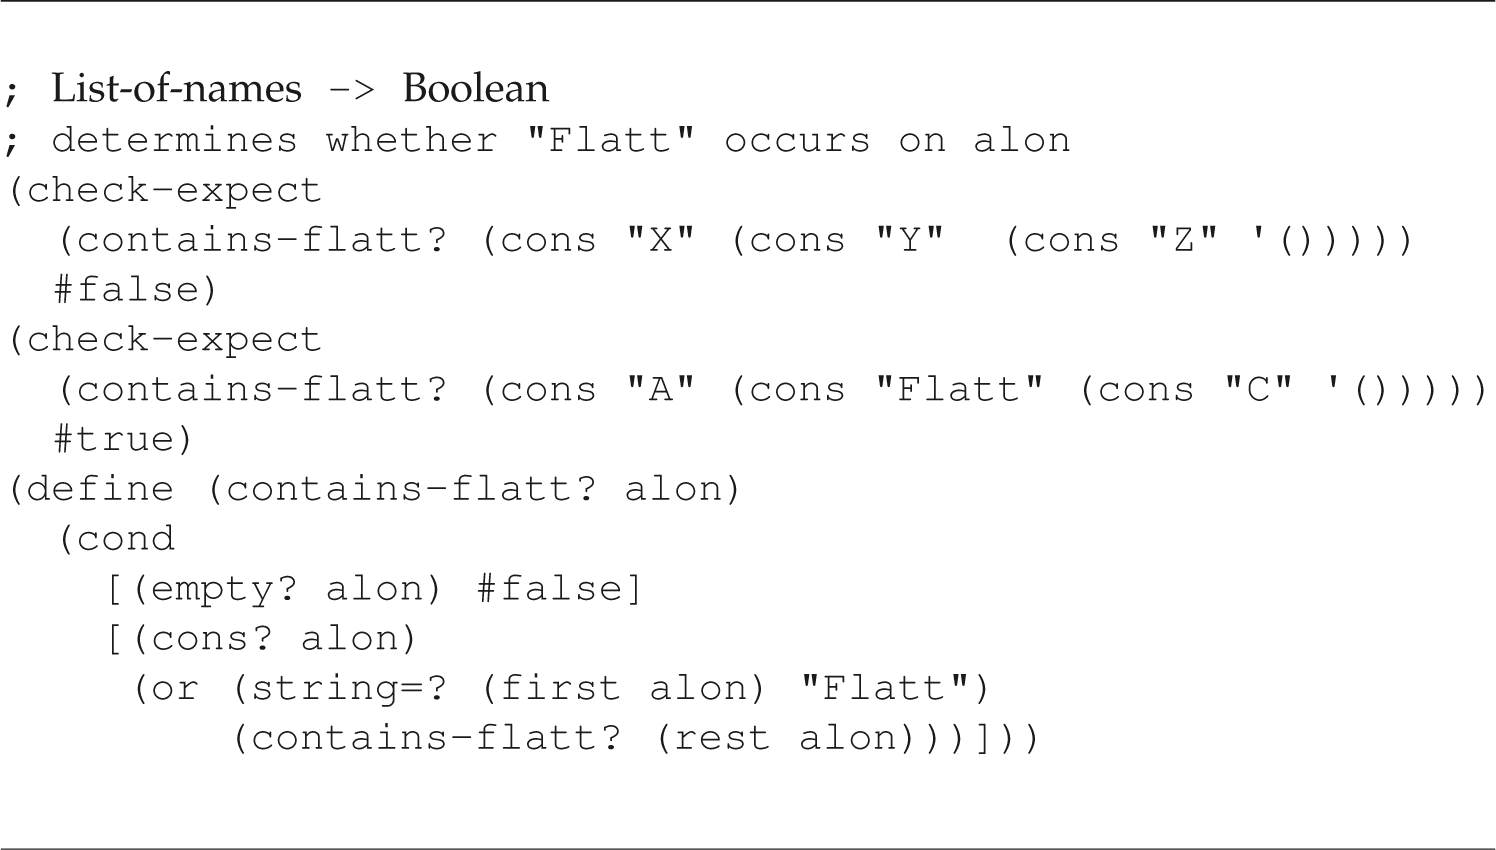
\includegraphics[width=0.85\textwidth]{images/00176.png}
  \caption{搜索列表}
  \label{fig:searching_a_list}
\end{figure}

\begin{exercise}{运行 contains-flatt?}{132}
在 DrRacket 中针对以下输入运行 \code{contains-flatt?}：
\begin{lstlisting}[language=BSL]
(cons "Fagan"
  (cons "Findler"
    (cons "Fisler"
      (cons "Flanagan"
        (cons "Flatt"
          (cons "Felleisen"
            (cons "Friedman" '())))))))
\end{lstlisting}
你预期的运行结果是什么？
\end{exercise}

\begin{exercise}{条件表达式的等价写法}{133}
下面是 \code{contains-flatt?} 中第二个 \code{cond} 分支的另一种表述方式：
\begin{lstlisting}[language=BSL]
(cond
  [(empty? alon) #false]
  [else
   (cond
     [(string=? (first alon) "Flatt") #true]
     [else (contains-flatt? (rest alon))])])
\end{lstlisting}
请解释为什么这个表达式与图~\ref{fig:searching_a_list} 中使用 \code{or} 的版本产生完全相同的结果。你认为哪个版本更好？请说明理由。
\end{exercise}

\begin{exercise}{通用查找函数 contains?}{134}
设计函数 \code{contains?}，判断给定的某个字符串是否出现在给定的字符串列表中。

\begin{notebox}[提示]
BSL 实际上内置了 \code{member?} 函数，它接受两个值并检查第一个值是否出现在作为列表的第二个值中：
\begin{replbox}
> (member? "Flatt" (cons "b" (cons "Flatt" '())))
#true
\end{replbox}
但在完成本练习时，\textbf{请不要}使用 \code{member?} 来定义 \code{contains?}。
\end{notebox}
\end{exercise}

\section{列表上的计算}
\label{sec:ch08_computing_with_lists}

由于我们仍在使用初学学生语言（BSL），代数求值规则（参见插曲 1）指导着我们如何在不借助 DrRacket 的情况下求出表达式的值，例如：
\begin{lstlisting}[language=BSL]
(contains-flatt? (cons "Flatt" (cons "C" '())))
\end{lstlisting}
程序员必须对此类代数演算过程拥有直观深刻的理解，因此我们逐步推演这个简单的例子。

图~\ref{fig:computing_with_lists_step1} 展示了第一步：应用常规的函数代换规则。结果是一个条件表达式，正如代数老师所说，该函数是以分段（step-wise）方式定义的。

\begin{figure}[htbp]
  \centering
  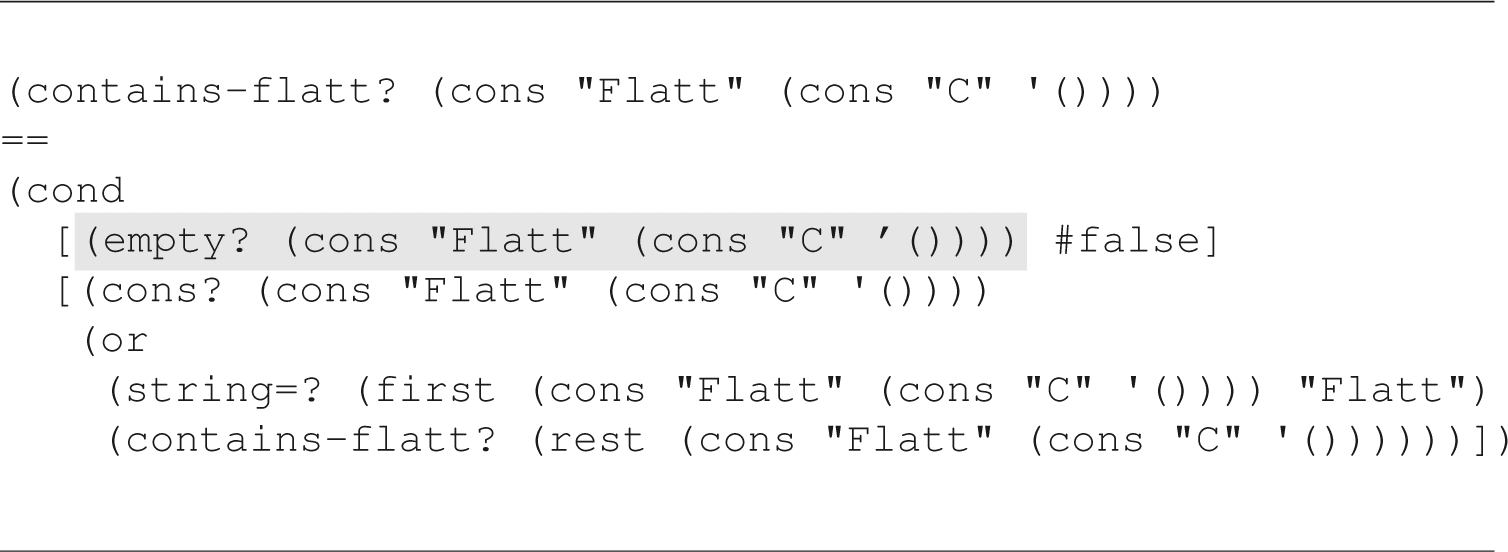
\includegraphics[width=0.85\textwidth]{images/00179.png}
  \caption{列表计算步骤 1}
  \label{fig:computing_with_lists_step1}
\end{figure}

图~\ref{fig:computing_with_lists_step2} 延续了这一演算过程。为了找到 \code{cond} 表达式的正确分支，我们必须逐一计算条件的值。由于 \code{cons} 构造出的列表不是空列表，第一个条件的值为 \code{\#false}，因此消去第一个 \code{cond} 分支。最后，第二个分支的条件求值为 \code{\#true}，因为对一个 \code{cons} 列表调用 \code{cons?} 必然成立。

\begin{figure}[htbp]
  \centering
  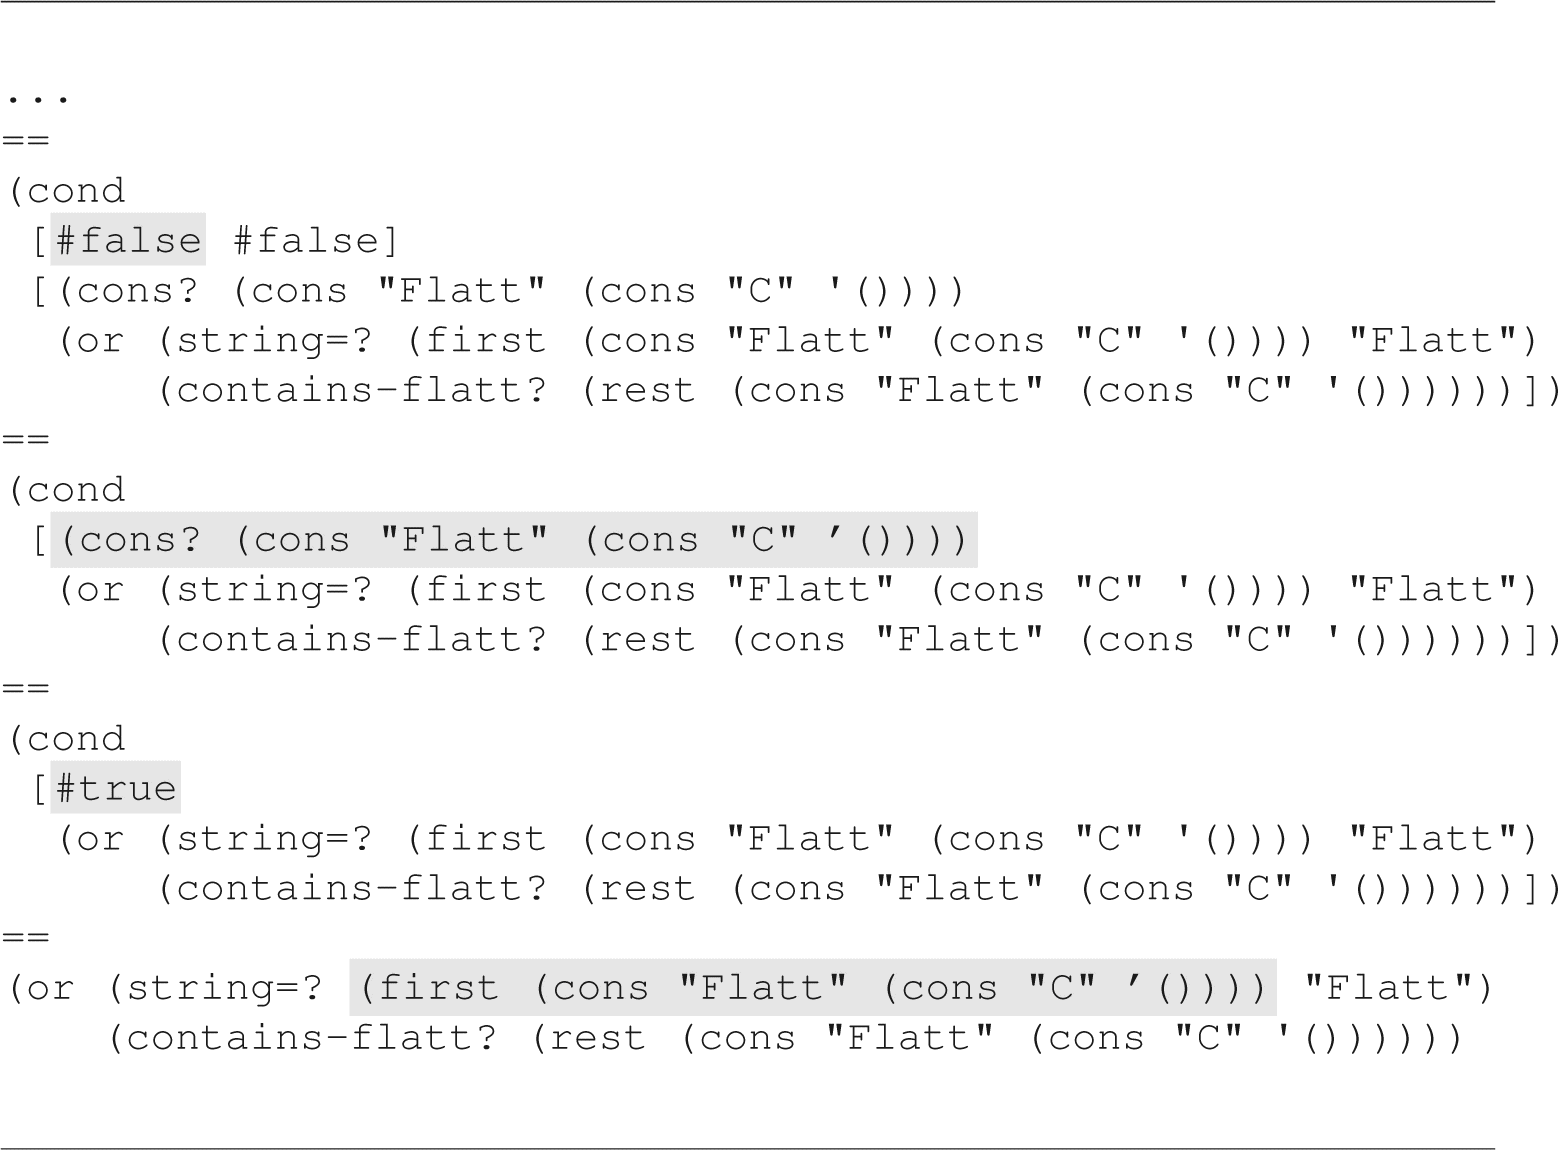
\includegraphics[width=0.85\textwidth]{images/00180.png}
  \caption{列表计算步骤 2}
  \label{fig:computing_with_lists_step2}
\end{figure}

从这里开始，仅需再经过三步基础算术化简即可得到最终结果。图~\ref{fig:computing_with_lists_step3} 展示了这三步：
\begin{enumerate}
  \item 根据 \code{first} 的求值法则，\code{(first (cons "Flatt" ...))} 被简化为 \code{"Flatt"}；
  \item 计算发现 \code{"Flatt"} 与 \code{"Flatt"} 确实是相等的字符串；
  \item 根据 \code{or} 的短路求值法则，无论表达式 $X$ 为何值，\code{(or \#true $X$)} 的结果都是 \code{\#true}。
\end{enumerate}

\begin{figure}[htbp]
  \centering
  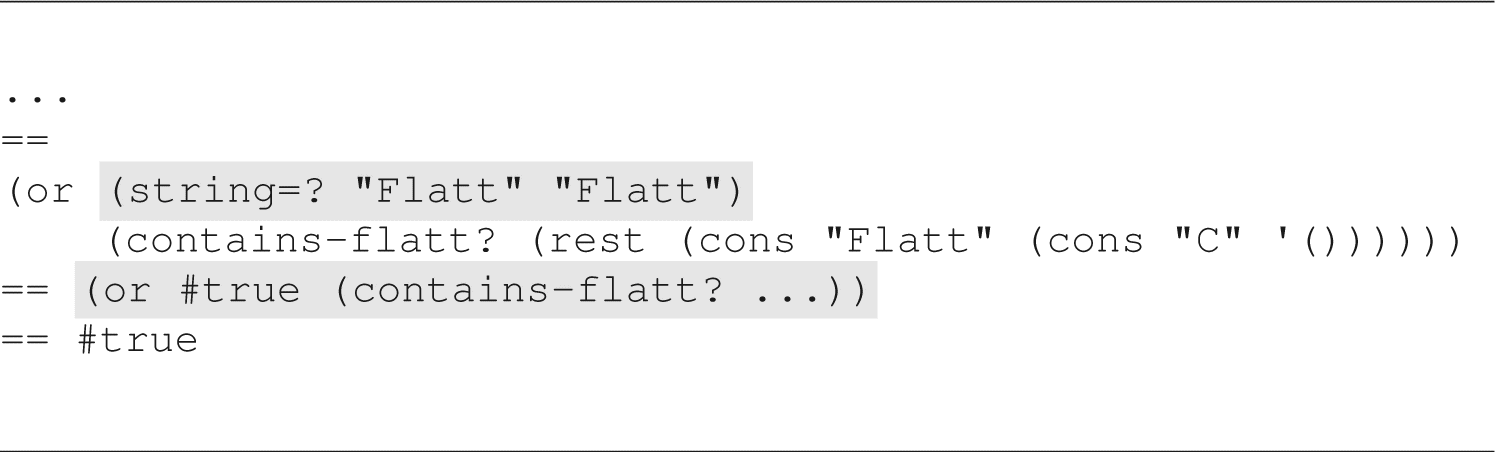
\includegraphics[width=0.85\textwidth]{images/00181.png}
  \caption{列表计算步骤 3}
  \label{fig:computing_with_lists_step3}
\end{figure}

\begin{exercise}{使用单步求值器观察 contains-flatt?}{135}
使用 DrRacket 的单步求值器（Stepper）单步观察以下表达式的计算过程：
\begin{lstlisting}[language=BSL]
(contains-flatt? (cons "Flatt" (cons "C" '())))
\end{lstlisting}
同时使用单步求值器观察下式的求值过程：
\begin{lstlisting}[language=BSL]
(contains-flatt? (cons "A" (cons "Flatt" (cons "C" '()))))
\end{lstlisting}
如果将 \code{"Flatt"} 替换为 \code{"B"} 会发生什么？
\end{exercise}

\begin{exercise}{验证列表原语选择器}{136}
利用 DrRacket 的单步求值器验证以下恒等关系：
\begin{lstlisting}[language=BSL]
(our-first (our-cons "a" '())) == "a"
(our-rest (our-cons "a" '())) == '()
\end{lstlisting}
有关这些函数的定义，请参见第 8.2 节。
\end{exercise}
